\cptr{Bayesian latent variable models for the analysis of experimental psychology data}
{Bayesian latent variable models}
{Edgar C.\ Merkle and Ting Wang}


\let\proglang=\textsf
\let\pkg=\emph
\let\code=\texttt

Traditional applications of factor analysis and related latent variable models include psychometric scale development, analysis of observational data, and possibly data reduction (though the related, but distinct, principal components analysis is more relevant here).  Because experimental psychologists do not typically embark on such applications, they may regard latent variable models as being irrelevant to their statistical toolboxes.  Furthermore, applications of latent variable models to experimental data are relatively uncommon in the literature \cite<though see>{bagyi89,don03,miy00,ruskah98,wicdol05}. In this paper, we illustrate  that Bayesian latent variable models can be advantageous for the analysis of multivariate data collected in many laboratory experiments.  The models flexibly allow us to handle data from multiple trials, conditions, or scenarios, without the need for aggregation across trials or subjects.  This allows us to pool data across multiple trials in order to draw general conclusions about the research question of interest, while preserving variability inherent in the raw data. We focus on Bayesian versions of the models because they are flexible and advantageous for model extension, comparison, and interpretation.

Bayesian approaches to estimating latent variable models have been considered for at least forty years, with increased attention to the subject following the computational advances in Markov chain Monte Carlo (MCMC).  Early treatments include \citeA{pre72}, \citeA{marmcd75}, \citeA{bar81}, and \citeA{lee81}, while later treatments that incorporate MCMC include \citeA{schhoi99}, \citeA{lee07}, \citeA{sonlee12}, and \citeA{mutasp12}.  Some authors of the recent papers refer to a need for fully automated software that fits latent variable models via MCMC, with \proglang{Mplus} \cite{mplus} providing SEM functionality and \proglang{BUGS} \cite{bugs12}, \proglang{JAGS} \cite{plu03}, and \proglang{Stan} \cite{stan14} providing general functionality.  This automation has the reward of easily estimating complex models coupled with the risk of estimating inappropriate models or drawing inappropriate conclusions \cite<also see>{macedw12,ste01,strmil14}.

In the pages below, we first present an overview of factor analysis and structural equation models.  We also discuss necessary topics for Bayesian model estimation, including prior distribution specification and model comparison methods. The Bayesian methods are trickier than they are for other models because of the inherent parameter identification issues.  We then apply the models to data from an experiment on risky choice, highlighting the unified and unique results that the models can provide.  We estimate all models in \proglang{JAGS} and carry out related computations in \proglang{R}; code to replicate all results is provided at the URL referenced at the end of the paper.


\section{Models}

To describe the models, we first set up a framework that is relevant to experimental research.  We assume that $n$ individuals respond to a series of stimuli that are all intended to measure the same concept.  Across the stimuli, each individual contributes $p$ observed variables.  For example, in the illustration later, the stimuli are five binary choices.  For each choice stimulus, individuals rate (i) the extent to which each individual choice option is attractive and (ii) the extent to which they prefer one stimulus over the other.  Here, the stimuli are all intended to measure an individual's attraction to risk, and each individual provides $p=15$ observed variables: three ratings for each of 5 stimuli.  We generally assume that $y_{ij}$ ($i=1,\ldots,n$; $j=1,\ldots,p$) is individual $i$'s response to observed variable $j$, and we also sometimes assume that individuals are randomly assigned to a between-subjects condition. This mimics many psychology experiments, where researchers are interested in studying whether experimental conditions impacted individuals' responses across multiple trials.

In the discussion below, we assume that $y_{ij}$ is approximately continuous (so that our models fully rely on normal distributions). However, variants of these models can also be applied to discrete data such as binary choices or ordinal ratings.  These variants are highly related to the item response models that are described in \citeA{bartl18}.
%a separate paper within this special issue. ({\color{red} we plan to cite the other paper once we see it.})

\subsection{Factor Model}

The traditional factor model \cite<e.g.,>{lawmax71,barkno11} assumes that each individual has a stable underlying trait (e.g., attraction to risky choice) across all experimental stimuli. An individual's response to each stimulus is driven by this trait. The stimuli are unique, however, so that stimulus characteristics also impact the individual's responses.  Further, like many other models, noise impacts the responses.

The above ideas can be formally represented by:
\begin{align} \label{eq:1fac}
    y_{ij} | \theta_i, \gamma_j, \lambda_j, \psi_j &\sim N(\mu_{ij}, \psi_j)\ \ \ \text{for all }i,j \\ \label{eq:1fmn}
    \mu_{ij} &= \gamma_j + \lambda_j \theta_i \\
    \theta_i &\sim N(0, \phi).
\end{align}
Within this model, $\theta_i$ is the value of individual $i$'s stable trait.  This value arises from a normal distribution with mean 0 and variance $\phi$, reflecting the distribution of the trait across the population of interest.  The observed response $y_{ij}$ is perturbed from the trait by the sources mentioned in the previous paragraph: stimulus characteristics $\gamma_j$ and $\lambda_j$, and random noise with variance $\psi_j$.  

The stimulus characteristics include the intercept $\gamma_j$, reflecting stimulus $j$'s mean response in the population of interest, and slope $\lambda_j$, reflecting the extent to which stimulus $j$ ``taps into'' the trait of interest.  If $\lambda_j$ equals 0, individual $i$'s standing on the trait has no impact on his/her response $y_{ij}$.  Conversely, if $\lambda_j$ is large (in the positive or negative direction), individual $i$'s standing on the trait has a large impact on his/her response.  In traditional applications, the $\lambda_j$ are called {\em factor loadings} and the trait of interest is called the {\em factor}.

\subsubsection{Multiple factors}

The above model assumed that a single latent trait was associated with the observed responses $y_{ij}$.  In some studies, multiple traits will have an association.  For example, undergraduate participants' responses to a recognition memory task may be influenced both by their working memory capacity and by their attentional functioning during the experiment.  If a participant has both high working memory and high attention, he/she should exhibit good test performance.  Conversely, low values of either trait will result in lower performance.

Assuming that $m$ traits impact observed responses, we can modify the previous model to arrive at an ``$m$-factor model:''
\begin{align} \label{eq:mfac}
    y_{ij} | \bm{\theta}_i, \gamma_j, \bm{\Lambda}_j, \psi_j &\sim N(\mu_{ij}, \psi_j)\ \ \ \text{for all }i,j \\ \label{eq:mfac2}
    \mu_{ij} &= \gamma_j + \displaystyle \sum_{k=1}^m \lambda_{jk} \theta_{ik} \\ \label{eq:mfact}
    \bm{\theta}_i &\sim N_m(\bm{0}, \bm{\Phi}),
\end{align}
where $\bm{\theta}_i$ is a vector describing individual $i$'s standing on each of the $m$ latent traits (with this vector now arising from a multivariate normal distribution) and $\bm{\Lambda}_j$ contains the $m$ factor loadings for stimulus $j$.  The matrix $\bm{\Phi}$ contains information about the variance of each trait along with covariances between pairs of traits.  For the next section, it is helpful to combine the $\bm{\Lambda}_j$ into a $p \times m$ matrix $\bm{\Lambda}$.  

\subsubsection{Exploratory versus confirmatory models} \label{sec:id}

From inspection of the above models, it is evident that there are some unidentified parameters.  For example, Equation~\eqref{eq:1fmn} involves the multiplication of two unknown parameters $\lambda_j \times \theta_i$.  If we multiply each $\lambda$ by a constant and divide each $\theta$ by the same constant, our model predictions remain unchanged.  This lack of identification is compounded by the fact that the $\bm{\Phi}$ matrix typically contains additional free parameters. To address problems such as this, we need to fix some model parameters to constants (typically to zero or one). Additionally, when we consider the $m$-factor model from Equations~\eqref{eq:mfac} to~\eqref{eq:mfact}, it is possible to use matrix algebra to illustrate a {\em rotational indeterminacy} problem. This implies that specific linear transformations (more complex than multiplication by a constant) of the $\lambda$ parameters, coupled with inverse transformations of the $\theta$ parameters, lead to unchanged model predictions.  

The $m$-factor model requires us to systematically constrain $m^2$ parameters in order to achieve identification (this does not count the mean of $\bm{\theta}_i$, which is fixed to $\bm{0}$).  If we constrain only the minimum $m^2$ parameters, we obtain an {\em exploratory} factor model. This model allows for the possibility that all latent traits (contained in $\bm{\theta}$) are associated with all observed measures (the $y_{ij}$). We can obtain unique parameter estimates based on the specific $m^2$ parameter constraints employed, but there are an infinite number of other, equally-good sets of parameter values coupled with alternative parameter constraints (these arise from the rotational indeterminacy issue described in the previous paragraph).  Because of this, the $\lambda$ (and possibly $\bm{\Phi}$) parameters are typically transformed following model specification so that they are easily interpretable.  This ``interpretability'' step is called {\em rotation}, and we provide some further information on it in the General Discussion \cite<also see>{bro01}. Regardless of the rotation step, however, the exploratory model can be useful because it allows us to compare models with different values of $m$.  This can provide information about the number of latent traits associated with the observed measures, as well as about which latent traits are associated with which measures.

If we fix more than $m^2$ parameters, we obtain a {\em confirmatory} factor model.  In this model, we assume that some latent traits have no association with some observed measures (consequently, some of the parameters in $\bm{\Lambda}$ are fixed to zero) and also assume fixed, nonzero values for some parameters.  Rotational indeterminacy is no longer a problem here, though alternative parameter constraints can still impact parameter estimates.  These are further described below.

\subsubsection{Identification constraints for factor models} \label{sec:id2}

Regardless of whether we have an exploratory or confirmatory model, the first $m^2$ parameter constraints must be set in a systematic fashion \cite<see>{jor69,jor79,pee12b,pee12} to identify the likelihood.  Popular strategies are described below; all strategies assume that the resulting $\bm{\Lambda}$ matrix is of full rank (e.g., that we cannot obtain one column of $\bm{\Lambda}$ through a linear combination of other columns) and that the resulting $\bm{\Phi}$ matrix is positive definite.

Often, we start by setting $\bm{\Phi} = \bm{I}$, which means that each latent trait has a variance of 1 with each pair of traits having a 0 correlation.  If we employ this constraint, we then systematically fix $m(m-1)/2$ parameters in $\bm{\Lambda}$: one column can have no zeros, one column must have one zero, one column must have two zeros, \ldots, and one column must have $(m-1)$ zeros.

Alternatively to above, we can fix the diagonal of $\bm{\Phi}$ (reflecting latent trait variances) to equal 1 but allow other parameters in $\bm{\Phi}$ to be unconstrained.  This allows for the possibility that latent traits are correlated.  If we opt for these constraints, we must fix more parameters in $\bm{\Lambda}$ to zero.  In particular, each column of $\bm{\Lambda}$ must now contain $(m-1)$ zeros, for a total of $m(m-1)$ zeroes in $\bm{\Lambda}$.  These restrictions, proposed by \citeA{jor79}, achieve ``local'' identification: they identify the model up to sign changes in columns of $\bm{\Lambda}$. \citeA{pee12} describes how to make these constraints globally identified: in addition to the above constraints, one must force a nonzero parameter in each column of $\bm{\Lambda}$ to assume only positive or negative values.  

Finally, another strategy involves placing all the restrictions in $\bm{\Lambda}$.  Now $\bm{\Phi}$ is completely unconstrained, with each column of $\bm{\Lambda}$ containing $(m-1)$ zeros.  Each column of $\bm{\Lambda}$ must also contain a nonzero constant, typically one (with each one appearing in different rows), compensating for the unconstrained $\bm{\Phi}$.  These restrictions, also proposed by \citeA{jor79}, achieve global identification.

The above constraints might make some readers uncomfortable, leading them to wonder whether estimated parameters can be interpreted given all the identification issues involved.  We suggest first comparing
exploratory models via Bayes factors (or other global model statistics), which should be approximately invariant to the specific identification constraints that are chosen. The Bayes factors will provide information about the best value of $m$ or about which latent traits impact which observed measures.  Interpretation of a single model may then proceed by studying the pattern of $\lambda$ estimates across latent traits and observed variables; see \citeA{hoyduv04,peedzi14}, and \citeA{premac03} for further discussion of related strategies.  In addition to these strategies, the models can be extended so that we obtain estimates of experiment-specific parameters.  This motivates the use of structural equation models, described later.

\subsubsection{Exploratory models and priors}
In ML contexts, one often fits the model to the observed covariances between the $p$ variables and integrates out the latent variables $\bm{\theta}$.  In Bayesian contexts, one typically fits the model to the raw data, and $\bm{\theta}$ is usually sampled simultaneously with other model parameters via MCMC.  This sampling of the latent variables introduces some identification issues that are specific to Bayesian factor models.  If these issues are not addressed, the sampled parameters will never converge to a stationary distribution.

To address the identification issues, we adopt a parameter expansion approach \cite{gel04,gel06,ghodun09} to fit exploratory factor models. Parameter expansion involves sampling from a ``working model'' with unidentified parameters.  At each iteration of the sampling, we transform the sampled parameters to correspond to the ``inferential model'' with uniquely identified parameters. This improves the speed at which the sampled chains converge to the posterior distribution, while also handling some of the parameter identification issues inherent to the model.

The working model is intended to help us sample the factor loadings $\lambda$ and the latent trait values $\theta$.  We allow the entire covariance matrix $\bm{\Phi}^*$ to be unconstrained, and we also fix $m(m-1)$ parameters in $\bm{\Lambda}^*$ to zero (see p.~\pageref{sec:id2}).  We then place the following prior distributions on the rest of the (unidentified) parameters:
\begin{align}  \label{eq:lampri}
    \lambda_{jk}^* &\sim N(0,1)\ \ \text{for }\lambda_{jk}^*\text{ free} \\
    \bm{\theta}_{i}^* &\sim N_m(\bm{0},\bm{\Phi})\ \ i=1,\ldots,n \\ \label{eq:phipri}
    \bm{\Phi}^{*-1} &\sim \text{Wishart}(\bm{V}, m),
\end{align}
where $\bm{V}$ is an $m \times m$ covariance matrix, and the asterisks on the $\theta$s, $\lambda$s, and $\phi$s imply that these parameters are unidentified.  At each iteration, these unidentified working parameters are transformed to identified versions in the inferential model via
\begin{align}
    \lambda_{jk} &= \text{sign}(\lambda_{kk}^*) \lambda_{jk}^* \phi^{*1/2}_{kk} \\
    \theta_{ik} &= \text{sign}(\lambda_{kk}^*) \phi^{*-1/2}_{kk} \theta^*_{ik} \\
    \phi_{k\ell} &= \frac{\text{sign}(\lambda_{kk}^*) \text{sign}(\lambda_{\ell\ell}^*) \phi^*_{k\ell}}{\sqrt{\phi^{*}_{kk} \phi^{*}_{\ell\ell}}},\ \ k,\ell=1,\ldots,m,
\end{align}
where $\text{sign}(\lambda_{kk}^*)$ equals either $1$ or $-1$, depending on whether $\lambda_{kk}^*$ is positive or negative. These transformations automatically yield the remaining constraints necessary to globally identify the model parameters: in addition to the $m(m-1)$ parameters of $\bm{\Lambda}$ fixed to zero, we now have that parameters along the diagonal of $\bm{\Phi}$ equal 1.  Further, we have restricted one parameter in each column of $\bm{\Lambda}$ to be positive, which is one way to fulfill the sign restriction described by \citeA{pee12}.  This procedure results in chains of sampled parameters that quickly converge to their posterior distributions for small values of $m$ (say, 5 or less).

For large values of $m$, the specific $\lambda$ parameters that are fixed to zero can impact convergence.  If these constraints cause the posterior associated with one of the $\lambda_{kk}$ to overlap with zero, then the chains cannot converge (because, under the parameter expansion approach, $\lambda_{kk}$ can only be positive).  This is only problematic if many of the observed variables are not associated with the latent traits of interest. 

\subsection{Structural Equation Models}
The factor model can be extended in a variety of ways, many of which are relevant to experimental psychologists.  For example, suppose that each participant $i$ is assigned to one of two experimental conditions. We can allow unique parameters for each condition, which can provide information about the extent to which the parameters differ across conditions \cite<e.g.,>{mil11,verfox13}.  These types of models are often called {\em multiple-group models}.

We can also allow specific latent traits to influence other latent traits.  For example, in situations where subjects choose between risky and riskless options, subjects' latent attractions to each type of option should influence their choice.  Models that include directional influences of latent traits on other latent traits are no longer factor models; they are instead {\em structural equation models}.  Structural equation models subsume factor models and can be written as
\begin{align} \label{eq:sem}
    y_{ij} | \bm{\theta}_i, \gamma_j, \bm{\Lambda}_j, \psi_j &\sim N(\mu_{ij}, \psi_j)\ \ \ \text{for all }i,j \\  \label{eq:sem2}
    \mu_{ij} &= \gamma_j + \displaystyle \sum_{k=1}^m \lambda_{jk} \theta_{ik} \\  \label{eq:sem3}
    \theta_{ik} &= \alpha_k + \displaystyle \sum_{\ell=1}^m B_{k\ell} \theta_{i\ell} + \zeta_{ik}\ \ \ \text{for all }i,k,
\end{align}
where $\alpha_k$ is the mean of latent trait $k$ (often fixed to zero) and $\zeta_{ik}$ is a normally-distributed, zero-centered residual term associated with latent trait $k$.  Equation~\eqref{eq:sem3} may
look confusing to some because the $\theta$ parameters appear on both sides of the equation.  This is the part of the equation that allows some latent traits to have directional influences on others.  We require $B_{kk}=0,\ k=1,\ldots,m$, which simply means that no latent trait exerts a directional influence on itself.  Many of the other $B$ parameters are also fixed to zero; the only nonzero $B$ parameters correspond to latent variables that have a directional influence on another latent variable.

Finally, the structural equation model presented above can be further extended to allow for interactions between latent variables \cite<e.g.,>{klemoo00}. To do so, we maintain most of the previous model, replacing only Equation~\eqref{eq:sem3} with
\begin{equation}
    \label{eq:semint}
    \theta_{ik} = \alpha_k + \displaystyle \sum_{\ell=1}^m B_{k\ell}
    \theta_{i\ell} + \displaystyle \sum_{q_1=1}^m \displaystyle
    \sum_{q_2=q_1}^m \xi_{kq_1q_2} \theta_{iq_1} \theta_{iq_2} + \zeta_{ik}\ \ \ \text{for all }i,k,
\end{equation}
where $\zeta_{ik}$ is still a zero-centered residual and many of the $\xi$ parameters are fixed to zero (as are many of the $B$ parameters).  This model is difficult to fit via ML methods and simpler to fit via Bayesian methods \cite{leeson07}.  Bayesian methods allow us to sample the latent variables $\bm{\theta}_i$, which in turn allow us to deal with the conditional distribution of $\bm{y}_i$ given $\bm{\theta}_i$.  These conditional distributions are normal, regardless of whether or not we employ latent variable interactions. In contrast, ML methods work on the marginal distribution of $\bm{y}_i$, integrating out the latent variable $\bm{\theta}_i$.  When there are latent variable interactions in the model, this marginal distribution is no longer normal.  Consequently, special ML estimation methods must be developed specifically for models that include latent variable interactions.  For more discussion of these issues and specific ML model estimation methods, see \citeA{cudhar09}, \citeA{klemoo00}, \citeA{klemut07}, and \citeA{marwen13}.

\subsubsection{Identification constraints for SEMs}
Structural equation models' likelihoods are identified when both the measurement part (Equation~\eqref{eq:sem2}) and the structural part (Equation~\eqref{eq:sem3}) are identified \cite{lee07}. Identification of the measurement part is typically handled in a manner similar to the factor analysis models. There exist no general rules for identifying the structural part, however \cite{bol09}.  Researchers approach this problem by satisfying some (not unique) sufficient conditions that are relatively easy to satisfy in practice \cite{lee07}.  These conditions often focus on {\em nonrecursive} relationships between latent variables, which include reciprocal directional effects, feedback loops, and correlated residuals.  The idea is that, to achieve identification, we should minimize the number of directional influences and covariances between latent variables (i.e., we want to avoid cases where most of the $B$ parameters are estimated and where the covariance matrix associated with $\zeta$ is nearly unrestricted).  See \citeA{rig95} for further discussion of these issues.

\subsubsection{SEMs and priors}
To specify the priors for structural equation models, we adopt an approach related to that described by \citeA{mer11}, \citeA{cur10}, and others.  We fix the latent variable variances $\phi$ to 1 and then, for each factor, restrict at least one loading $\lambda$ to have a prior distribution that is truncated from below at 0.  This truncation solves the ``sign change'' issue that was described by \citeA{pee12}.  We could also use a parameter expansion approach here, but it adds extra complexity to the already-complex JAGS code.  Further details on this issue, along with specific prior distributions used, appears in the Application section.  For the JAGS code used to fit the models, see the Computational Details section at the end of the paper.


\section{Model Comparison: Bayes Factor Computation}

In a latent variable context, Bayes factors are useful for comparing models with differing numbers of latent traits (i.e., models with different values of $m$) or for comparing structural equation models with different covariates.  We compute log-Bayes factors to compare pairs of models in this paper, with positive values generally conveying support for more complex models (which contain extra effects or factors).  \citeA{kasraf95} provide some rules of thumb for their interpretation, suggesting that log-Bayes factors below 1 are ``not worth more than a bare mention,'' values from 1 to 3 are ``positive,'' values from 3 to 5 are ``strong,'' and values greater than 5 are ``very strong.''   Like most rules of thumb, these values are subject to debate.

To compare models with different values of $m$, factor analysts have traditionally used the method of path sampling for Bayes factor computation \cite{leeson02,ghodun09}.  This method was originally described by \citeA{gelmen98}, but recent work suggests that it can be problematic when it is applied to factor analysis \cite{dutgho13}.  Hence, we rely on the Laplace approximation to the Bayes factor \cite{kasraf95,lewraf97}, and we also use the Savage-Dickey method \cite{diclie70,wag10} to check our results.  We now briefly describe the Laplace approximation and the Savage-Dickey density ratio.  Alternative methods for computing Bayes factors are described by, e.g., \citeA{kasraf95}, \citeA{lopwes04}, \citeA{roumor12}, and \citeA{roumor12b}.

\subsection{Laplace Approximation}
The Laplace approximation to the Bayes factor (which we use throughout the paper) is used to approximate the integrals involved in the candidate models' marginal likelihoods (the ratio of which yields the Bayes factor). Given a model, the Laplace approximation to the marginal log-likelihood is \cite{lewraf97}
\begin{equation} \label{eq:lapapp}
    \log( f(\bm{Y})) \approx \frac{q}{2} \log(2\pi) + \frac{1}{2} \log(|\bm{J}^{-1*}|) + \log( f(\bm{\Omega}^*)) + \log( f(\bm{Y} | \bm{\Omega}^*)),
\end{equation}
where $\bm{\Omega}$ is the model parameter vector of length $q$, $\bm{\Omega}^*$ is a posterior central tendency measure of $\bm{\Omega}$, $\bm{J}^{-1*}$ is the inverse of the information matrix evaluated at $\bm{\Omega}^*$, and $f()$ is the probability distribution of the terms within its parentheses. This approximation has been found to be accurate when the posterior distribution is unimodal without long tails \cite{lewraf97,tiekad86}, and its error in approximating the Bayes factor is of order $O(n^{-1})$ \cite{kasraf95}.  \citeA{raf93} has previously considered the approximation's application to the types of models described here.

The beauty of the Laplace approximation involves the fact that all four terms on the right of~\eqref{eq:lapapp} can often be obtained directly from MCMC output.  The first term is trivial.  The second term can be estimated via the covariance matrix of sampled parameters.  The third term requires $\bm{\Omega}^*$, which is a posterior central tendency measure of each sampled parameter (and we are evaluating the prior distributions at $\bm{\Omega}^*$).  Finally, the fourth term requires us to evaluate the likelihood at $\bm{\Omega}^*$.  

The fourth term can be somewhat difficult to evaluate when there are random effects in the model that are not officially counted as model parameters; this includes the $\bm{\theta}$ parameters in the factor models described here. As \citeA{lewraf97} describe, we must integrate out the random effects in order to calculate the fourth term.  This is easy to do for factor models involving normal distributions because we can solve the integral analytically.  The solution is:
\begin{equation} \label{eq:factor}
    \bm{y}_i | \bm{\gamma}, \bm{\Lambda}, \bm{\Phi}, \bm{\Psi} \sim  N_p(\bm{\gamma}, \bm{\Lambda \Phi \Lambda}^\prime + \bm{\Psi}),
\end{equation}
where $\bm{y}_i$ is individual $i$'s data vector, $\bm{\gamma}$ is a vector of intercepts, $\bm{\Psi}$ is a diagonal matrix of residual variances, and $\bm{\Lambda}$ (the collection of factor loadings) and $\bm{\Phi}$ (the latent trait covariance matrix) were defined previously.  For SEMs involving normal distributions the solution is 
\begin{equation}
  \bm {y}_i | \bm \gamma, \bm \Lambda, \bm \Phi, \bm \Psi, \bm \alpha, \bm B, \bm \Delta \sim 
  N_p(\bm \gamma+\bm \Lambda \bm \alpha, \bm \Lambda \bm B \bm \Phi \bm{B}^\prime \bm{\Lambda}^\prime + \bm \Lambda \bm \Delta \bm
  \Lambda^{\prime} + \bm \Psi),
\end{equation}
where $\bm {y}_i, \bm \gamma, \bm \Lambda$ and $\bm \Psi$ are defined in the same way as Equation~\eqref{eq:factor}; $\bm \alpha$ is a vector of latent trait means; $\bm B$ is a matrix containing the $B$ parameters from Equation~\eqref{eq:sem3}; and $\bm \Delta$ is a matrix containing the variances of the residual terms $\bm \zeta_{ik}$ from Equation~\eqref{eq:sem3}.  The matrix $\bm \Phi$ is still the latent trait covariance matrix, but the vital difference between SEM and factor analysis involves the entries of $\bm \Phi$.  In factor analysis, each entry of $\bm \Phi$ is either a single parameter or a constraint (0 or 1).  In SEMs, we need to derive many entries of $\bm \Phi$ via conditional distributions.  This is one reason why the Bayesian SEM framework can be extended more flexibly. For example, for latent variable interactions, we can separate observed variables that ``receive'' a latent interaction from those that do not, then rely on the conditional distribution of the former observed variables (conditioned on the other latent variables) to arrive at the full marginal distribution. If our models involve distributions other than the normal (as is the case for, say, logistic regressions and many item response models), then integration of the random effects is less straightforward.  Further MCMC steps could be used here; see \citeA{lewraf97} for more detail.

\subsection{Savage-Dickey Density Ratio}
The Savage-Dickey density ratio is useful for computing Bayes factors associated with nested models; such models often mimic null hypotheses.  In such situations, we often wish to test a hypothesis that a model parameter (or some function of model parameters) equals zero.  We can gain information related to this hypothesis by comparing two models: Model A, where the parameter in question is freely estimated, and Model B, where the parameter in question is constrained to zero.  In computing a Bayes factor to compare these models, we gain information related to the chance that the model parameter actually equals zero.

The Savage-Dickey density ratio allows us to compute these types of Bayes factors by estimating only Model A (where the focal parameter is free).  Assume that we wish to calculate the Bayes factor associated with $\omega = 0$ versus $\omega \neq 0$, where $\omega$ is a specific entry of the parameter vector $\bm{\Omega}$.  Then we have that
\begin{equation}
    \label{eq:sdbf}
    BF_{BA} = \frac{p(\omega=0 | \bm{Y})}{p(\omega=0)};
\end{equation}
that is, the Bayes factor is the ratio between the posterior density evaluated at $\omega=0$ and the prior density evaluated at $\omega=0$.  The prior density is known, and the posterior density becomes normal for large $n$ \cite<e.g.,>{gelcarste04}.  For smaller $n$, the posterior density can be approximated via splines or kernel-based methods; see \citeA{wag10} for more detail.  Regardless, we can evaluate the posterior density using the MCMC output and a minimal amount of extra computation.

Throughout the application below, we report Bayes factors calculated via the Laplace approximation.  We also used the Savage-Dickey method to ensure that both methods agreed; while the Savage-Dickey methods are not reported here, the code used to calculate all Bayes factors is included in the replication code.  We now move to the application, which can be viewed as the start of a serious data analysis.

\section{Application: Risky Choice}

\citeA{petlev08} studied framing effects of risky and riskless choice alternatives in variants of the Asian Disease Problem \cite{tvekah81}.  This problem requires subjects to choose between two treatments for a fictional disease that impacts 600 people.  In a ``positive frame'' version of the problem, a riskless treatment saves 200 lives, while a risky treatment saves all 600 lives with probability 1/3 and no lives with probability 2/3.  In a ``negative frame'' version of the problem, a riskless treatment causes 400 people to die, while a risky treatment causes 0 deaths with probability 1/3 and 600 deaths with probability 2/3.  The question framing (number dead versus number alive) is known to have an impact on choice: ``death'' phrasing causes people to choose the risky option, while ``alive'' phrasing causes people to choose the riskless option.

\citeA{petlev08} were interested in the extent to which each option's attractiveness influenced choice, along with the impact of numeracy on the relationship between attractiveness and choice.  They created five variants of the Asian Disease Problem involving human deaths due to disease, animal deaths due to wildfire, and crop loss due to drought.  Subjects were assigned to one of two ``frame'' conditions, where the problems were phrased as described above.  Subjects reported a preference between options on a seven-point scale (from ``much prefer the riskless option'' to ``much prefer the risky option''), and they also rated the attractiveness of each option.  Thus, for each problem, subjects gave three ratings on seven-point scales: attraction to the risky option, attraction to the riskless option, and preference.  For each subject, the data therefore include 10 attractiveness ratings (of the risky option and the riskless option for each of the five problems) and 5 preference ratings (for each of the five problems). These ratings are all treated as continuous below, though similar models could be specified if, e.g., choice were binary.

The original authors' focal hypothesis was that  subjects' numeracy would moderate the relationship between attractiveness ratings and choice: as numeracy increases, attractiveness ratings should be more predictive of choice.   To study this hypothesis, the authors employed separate ANOVAs on each of the five problem variants and on data that were averaged over the problems.  They generally found statistically significant interaction effects in agreement with their focal hypothesis. In the analysis described here, we employ factor models and structural equation models to simultaneously  study the experimental data across all five problems and to handle potential differences between problems.  

\begin{figure}[p]
    \centering
    \usetikzlibrary{decorations.pathmorphing,backgrounds,fit,calc,through,arrows,shapes,trees,positioning,matrix,chains}
\tikzset {crossline/.style={opacity=.15,line width=4.5mm,line cap=round,color=#1},
	method/.style={opacity=.15,fill,rounded corners,color=blue},
	manifest/.style={rectangle,draw,inner sep=0.15em,minimum size=2.5em},
	latent/.style={circle,draw,inner sep=0.15em,minimum size=2.7em},
	error/.style={circle,draw,inner sep=0.15em,minimum size=2em},
	every loop/.style={min distance=1em,in=70,out=110,looseness=3.5},
	highlight/.style={rectangle,rounded corners,fill=red!15,draw,fill opacity=0.5,thick,inner sep=0pt}
}


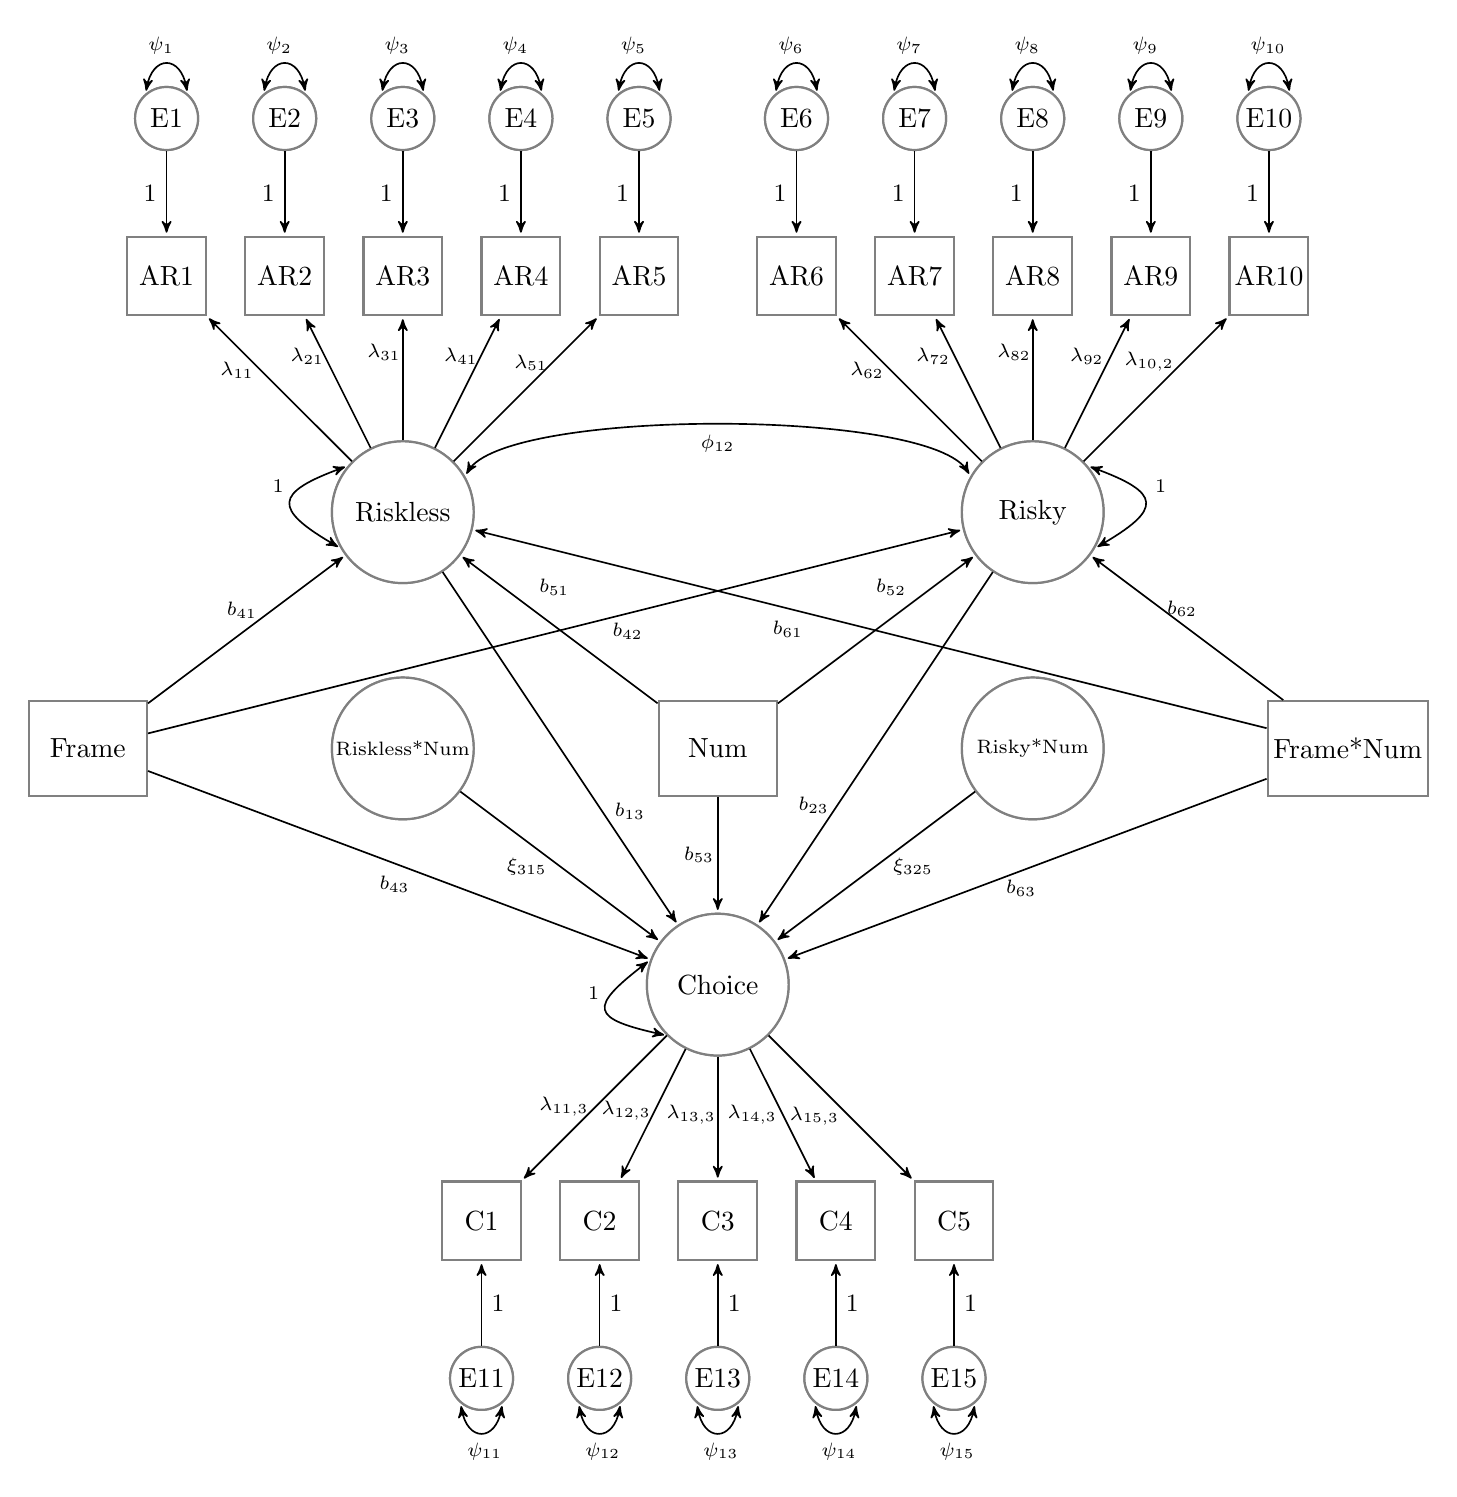
\begin{tikzpicture}
[latent/.style={circle,draw=black!50,fill=white!20,thick,
                inner sep=0pt, minimum width=18mm, 
                minimum height=18mm},
 manifest/.style={rectangle,draw=black!50,fill=white!20,thick,
                inner sep=0pt,minimum width=10mm, minimum height=10mm},
 covarite/.style={rectangle,draw=black!50,fill=white!20,thick,
                inner sep=2pt,minimum width=15mm, minimum height=12mm},
 error/.style={circle,draw=black!50,fill=white!20,thick,
                inner sep=0pt, minimum width=8mm},
 post/.style={->,shorten >=1pt,>=stealth',semithick},
 slingdash/.style={<->,shorten >=1pt,>=stealth',shorten
   <=1pt,>=stealth',auto, distance=9mm,dashed,semithick},
 sling/.style={<->,shorten >=1pt,>=stealth',shorten <=1pt,>=stealth',auto,distance=10mm,semithick},
 errorsling/.style={<->,shorten >=1pt,>=stealth',shorten <=1pt,>=stealth',auto,distance=5mm,semithick}]



%position objects.
\node[manifest] (AR1) at (-3,3) {AR1};
\node[manifest] (AR2) at (-1.5,3) {AR2};
\node[manifest] (AR3) at (0,3) {AR3};
\node[manifest] (AR4) at (1.5,3) {AR4};
\node[manifest] (AR5) at (3,3) {AR5};

\node[manifest] (AR6) at (5,3) {AR6};
\node[manifest] (AR7) at (6.5,3) {AR7};
\node[manifest] (AR8) at (8,3) {AR8};
\node[manifest] (AR9) at (9.5,3) {AR9};
\node[manifest] (AR10) at (11,3) {AR10};

\node[manifest] (C1) at (1,-9) {C1};
\node[manifest] (C2) at (2.5,-9) {C2};
\node[manifest] (C3) at (4,-9) {C3};
\node[manifest] (C4) at (5.5,-9) {C4};
\node[manifest] (C5) at (7,-9) {C5};

\node[covarite] (Frame) at (-4,-3) {Frame};
\node[covarite] (Num) at (4,-3) {Num};
\node[covarite] (Frame*Num) at (12,-3) {Frame*Num};

\node[latent] (Riskless) at (0,0) {Riskless};
\node[latent] (Risky) at (8,0) {Risky};
\node[latent] (Choice) at (4,-6) {Choice};
\node[latent] (Riskless*Num) at (0,-3) {\scriptsize{Riskless*Num}};
\node[latent] (Risky*Num) at (8,-3) {\scriptsize{Risky*Num}};

\node[error] (E1) at (-3,5) {E1};
\node[error] (E2) at (-1.5,5) {E2};
\node[error] (E3) at (0,5) {E3};
\node[error] (E4) at (1.5,5) {E4};
\node[error] (E5) at (3,5) {E5};

\node[error] (E6) at (5,5) {E6};
\node[error] (E7) at (6.5,5) {E7};
\node[error] (E8) at (8,5) {E8};
\node[error] (E9) at (9.5,5) {E9};
\node[error] (E10) at (11,5) {E10};

\node[error] (E11) at (1,-11) {E11};
\node[error] (E12) at (2.5,-11) {E12};
\node[error] (E13) at (4,-11) {E13};
\node[error] (E14) at (5.5,-11) {E14};
\node[error] (E15) at (7,-11) {E15};

%arrows, slings and texts
\node[latent] (Riskless) at (0,0) {Riskless}
   edge [post] node[above=0.01cm,text width=1.5cm]{\scriptsize{$\lambda_{11}$}} (AR1)
   edge [post] node[above=0.1cm,text width=1.2cm]{\scriptsize{$\lambda_{21}$}} (AR2)
   edge [post] node[above=0.1cm,text width=0.9cm]{\scriptsize{$\lambda_{31}$}} (AR3)
   edge [post] node[above=0.1cm,text width=0.6cm]{\scriptsize{$\lambda_{41}$}} (AR4)
   edge [post] node[above=0.1cm,text width=0.3cm]{\scriptsize{$\lambda_{51}$}} (AR5)
   edge [post] node[below right=0.8cm,text width=0.2cm]{\scriptsize{$b_{13}$}} (Choice)
  (Riskless.30) edge [sling,bend left=60]
   node[auto,swap]{\scriptsize{$\phi_{12}$}}(Risky.150)
  (Riskless.140) edge [sling,bend right=65]node[above left=0.05mm,text width=0.1cm]{\scriptsize{1}}(Riskless.210);

\node[latent] (Risky) at (8,0) {Risky}
   edge [post] node[above=0.01cm,text width=1.5cm]{\scriptsize{$\lambda_{62}$}} (AR6)
   edge [post] node[above=0.1cm,text width=1.3cm]{\scriptsize{$\lambda_{72}$}} (AR7)
   edge [post] node[above=0.1cm,text width=0.9cm]{\scriptsize{$\lambda_{82}$}} (AR8)
   edge [post] node[above=0.1cm,text width=0.7cm]{\scriptsize{$\lambda_{92}$}} (AR9)
   edge [post] node[above=0.1cm,text width=0.8cm]{\scriptsize{$\lambda_{10,2}$}} (AR10)
   edge [post] node[below left= 0.7cm,text
     width=0.35cm]{\scriptsize{$b_{23}$}} (Choice)
   (Risky.40) edge [sling,bend left=65]node[above right=0.05mm,text width=0.1cm]{\scriptsize{1}}(Risky.330)
;
   
\node[latent] (Riskless*Num) at (0,-3) {\scriptsize{Riskless*Num}}
   edge [post] node[left=0.05cm,text width=0.5cm]{\scriptsize{$\xi_{315}$}} (Choice)
   ;

\node[latent] (Risky*Num) at (8,-3) {\scriptsize{Risky*Num}}
   edge [post] node[right=0.1cm,text width=1.5cm]{\scriptsize{$\xi_{325}$}} (Choice)
   ;
  
   
\node[latent] (Choice) at (4,-6) {Choice}
   edge [post] node[above=-0.23cm,text width=1.4cm]{\scriptsize{$\lambda_{11,3}$}} (C1)
   edge [post] node[above=-0.2cm,text width=1.3cm]{\scriptsize{$\lambda_{12,3}$}} (C2)
   edge [post] node[above=-0.2cm,text width=1.3cm]{\scriptsize{$\lambda_{13,3}$}} (C3)
   edge [post] node[above=-0.25cm,text width=1.4cm]{\scriptsize{$\lambda_{14,3}$}} (C4)
   edge [post] node[above=-0.35cm,text width=1.3cm]{\scriptsize{$\lambda_{15,3}$}} (C5)
   edge [sling,bend left=65]node[above left=0.05mm,text width=0.1cm]{\scriptsize{1}}(Choice.160);
   
\node[covarite] (Frame) at (-4,-3) {Frame}
   edge [post] node[above=0.01cm,text width=0.5cm]{\scriptsize{$b_{41}$}} (Riskless)
   edge [post] node[right=0.6cm,text width=0.5cm]{\scriptsize{$b_{42}$}} (Risky)
   edge [post] node[below=0.01cm,text width=0.5cm]{\scriptsize{$b_{43}$}} (Choice);
   
\node[covarite] (Frame*Num) at (12,-3) {Frame*Num}
   edge [post] node[left=0.6cm,text width=0.5cm]{\scriptsize{$b_{61}$}} (Riskless)
   edge [post] node[above=0.01cm,text width=0.5cm]{\scriptsize{$b_{62}$}} (Risky)
   edge [post] node[below=0.01cm,text width=0.5cm]{\scriptsize{$b_{63}$}} (Choice);
   
\node[covarite] (Num) at (4,-3) {Num}
   edge [post] node[above =0.3cm,text width=0.5cm]{\scriptsize{$b_{51}$}} (Riskless)
   edge [post] node[above=0.3cm,text width=0.01cm]{\scriptsize{$b_{52}$}} (Risky)
   edge [post] node[left=0.05cm, text width=0.25cm]{\scriptsize{$b_{53}$}} (Choice)
  ;
   
\node[error] (E1) at (-3,5) {E1}
   edge [post] node[auto,swap]{\small{1}}(AR1)
   edge [errorsling, bend right= 80]node[above left=0.05mm,text width=0.1cm]{\scriptsize{$\psi_{1}$}} (E1.130);   
\node[error] (E2) at (-1.5,5) {E2}
   edge [post] node[auto,swap]{\small{1}}(AR2)
   edge [errorsling, bend right= 80]node[above left=0.05mm,text width=0.1cm]{\scriptsize{$\psi_{2}$}} (E2.130);
\node[error] (E3) at (0,5) {E3}
   edge [post] node[auto,swap]{\small{1}}(AR3)
   edge [errorsling, bend right= 80]node[above left=0.05mm,text width=0.1cm]{\scriptsize{$\psi_{3}$}} (E3.130);
\node[error] (E4) at (1.5,5) {E4}
   edge [post] node[auto,swap]{\small{1}}(AR4)
   edge [errorsling, bend right= 80]node[above left=0.05mm,text width=0.1cm]{\scriptsize{$\psi_{4}$}} (E4.130);
\node[error] (E5) at (3,5) {E5}
   edge [post] node[auto,swap]{\small{1}}(AR5)
   edge [errorsling, bend right= 80]node[above left=0.05mm,text width=0.1cm]{\scriptsize{$\psi_{5}$}} (E5.130);
\node[error] (E6) at (5,5) {E6}
   edge [post] node[auto,swap]{\small{1}}(AR6)
   edge [errorsling, bend right= 80]node[above left=0.05mm,text width=0.1cm]{\scriptsize{$\psi_{6}$}} (E6.130);
\node[error] (E7) at (6.5,5) {E7}
   edge [post] node[auto,swap]{\small{1}}(AR7)
   edge [errorsling, bend right= 80]node[above left=0.05mm,text width=0.1cm]{\scriptsize{$\psi_{7}$}} (E7.130);
\node[error] (E8) at (8,5) {E8}
   edge [post] node[auto,swap]{\small{1}}(AR8)
   edge [errorsling, bend right= 80]node[above left=0.05mm,text width=0.1cm]{\scriptsize{$\psi_{8}$}} (E8.130);
\node[error] (E9) at (9.5,5) {E9}
   edge [post] node[auto,swap]{\small{1}}(AR9)
   edge [errorsling, bend right= 80]node[above left=0.05mm,text width=0.1cm]{\scriptsize{$\psi_{9}$}} (E9.130);
\node[error] (E10) at (11,5) {E10}
   edge [post] node[auto,swap]{\small{1}}(AR10)
   edge [errorsling, bend right= 80]node[above left=0.05mm,text width=0.1cm]{\scriptsize{$\psi_{10}$}} (E10.130);
\node[error] (E11) at (1,-11) {E11}
   edge [post] node[auto,swap]{\small{1}}(C1)
   edge [errorsling, bend right= 80]node[below left=0.05mm,text width=0.05cm]{\scriptsize{$\psi_{11}$}} (E11.310);
\node[error] (E12) at (2.5,-11) {E12}
   edge [post] node[auto,swap]{\small{1}}(C2)
   edge [errorsling, bend right= 80]node[below left=0.05mm,text width=0.05cm]{\scriptsize{$\psi_{12}$}} (E12.310);
\node[error] (E13) at (4,-11) {E13}
   edge [post] node[auto,swap]{\small{1}}(C3)
   edge [errorsling, bend right= 80]node[below left=0.05mm,text width=0.05cm]{\scriptsize{$\psi_{13}$}} (E13.310);
\node[error] (E14) at (5.5,-11) {E14}
   edge [post] node[auto,swap]{\small{1}}(C4)
   edge [errorsling, bend right= 80]node[below left=0.05mm,text width=0.05cm]{\scriptsize{$\psi_{14}$}} (E14.310);
\node[error] (E15) at (7,-11) {E15}
   edge [post] node[auto,swap]{\small{1}}(C5)
   edge [errorsling, bend right= 80]node[below left=0.05mm,text width=0.05cm]{\scriptsize{$\psi_{15}$}} (E15.310);
   
\end{tikzpicture}

    \caption{Path diagram of the structural equation model used in the application.} \label{fig:em1:path}
\end{figure}

\subsection{Methods}
 We propose the use of factor analysis and SEM to study the authors' original hypotheses.  This allows us to draw unified inferences about the full experimental data from a single model, removing the need to do separate analyses of each problem.  While the modeling here can be viewed as the start of a full analysis, we omit some steps and issues due to space.  We further describe these omissions in the Discussion section.

Our modeling proceeds in two steps.  First, we fit 1- and 2-factor models (i.e., Equations~\eqref{eq:mfac} to~\eqref{eq:mfact}, with $m=1$ and $m=2$) to the ten attractiveness ratings given by each subject (one risky rating and one riskless rating, for each of the five questions).   The factors (latent variables) represent participants' attractions to risky and riskless alternatives in the context of this experimental study; they are used here to pool information across all five problems. In comparing a one-factor model to a two-factor model, we obtain information  about the nature of attraction to risky and riskless alternatives: are these two extremes of a continuum, or are they unique dimensions?  The former implies that a person who is attracted to risky alternatives is also repelled by riskless alternatives, while the latter implies that a person can be simultaneously attracted to (or repelled by) both risky and riskless alternatives.  This comparison provides information about the best way to model the effect of attractiveness ratings on choice.  To preview our results, we find that the 2-factor model is better than the 1-factor model.

 Next, we build off the results of the first step to examine the effects of risky/riskless attraction on choice, as well as to draw inferences related to the experimental manipulations and to numeracy. The model is most easily conceptualized via the path diagram in Figure~\ref{fig:em1:path}.  This diagram illustrates a series of regression-like relationships (directed arrows) between observed variables (squares) and latent traits (circles).  The observed variables AR1 to AR5 represent riskless attraction ratings for items 1--5; the observed variables AR6 to AR10 represent risky attraction ratings for items 6--10; and the observed variables C1 to C5 represent choice ratings for items 1--5.  Double-headed arrows imply variance parameters.

The base portion of the model involves three main latent variables: a riskless variable representing the riskless attraction ratings, a risky variable representing the risky attraction ratings, and a choice variable representing the choice ratings.  The experimental manipulation (frame), numeracy, and a frame-by-numeracy interaction predict all three of the main latent variables.  Finally, there appear two latent interaction variables: one between riskless attraction and numeracy, and one between risky attraction and numeracy.  These are notable because (i) they help us study the original authors' focal hypotheses, and (ii) interactions involving latent variables are difficult to estimate via ML methods.

 All observed variables are assumed to be conditionally normal, so that the path diagram can also be written as a combination of Equations~\eqref{eq:sem},~\eqref{eq:sem2}, and~\eqref{eq:semint}.  The parameter subscripts in Figure~\ref{fig:em1:path} match the subscripts that would be used in the equation version of the model (not shown). Additionally, to obtain the interactions from Equation~\eqref{eq:semint}, we implicitly create a latent numeracy variable that is perfectly related to the observed numeracy variable.

Prior distributions on model parameters are generally taken to be non-informative.  For the factor analysis models, many of the prior distributions are listed in Equations~\eqref{eq:lampri} to~\eqref{eq:phipri}.  The remaining parameters include the intercepts associated with observed variables ($\gamma_j$) and residual variances ($\psi_j$); these classes of parameters are assigned priors of
\begin{align}
    \gamma_j &\sim N(0, 10^3) \\
    \psi_j &\sim \text{Inv-Gamma}(0.1,0.1), 
\end{align}
where $j=1, 2, \ldots, 15$.  The $\gamma_j$ parameters are given exceptionally-large variances because they are essentially nuisance parameters here.  They represent the mean of each observed variable and play little role in the parameters of interest, which include the $\lambda_{jk}$, $\phi_{12}$, and $\psi_{j}$ parameters, where $j=1, 2, \ldots, 15;\ k=1, \ldots, 6$.  For completeness, note that the variances of the three observed covariates (labeled ``Frame,'' ``Num,'' and ``Frame by Num'') are fixed to their sample estimates.

For the structural equation model in Figure~\ref{fig:em1:path}, the $b_{k\ell}$ and $\xi_{kq_{1}q_{2}}$ parameters (paths between latent variables) can be somewhat difficult to sample.  This is because, for these parameters, the chains sampled via JAGS (and related software) exhibit high autocorrelation.  When the prior variances are very large, the MCMC algorithm can accept a ``bad'' posterior value, and the high autocorrelation implies that it will take a long time for the chain to recover from that bad value.  As a result, we use ``weakly informative'' prior distributions on the parameters \cite{gel06}: prior distributions with variances constrained to reflect plausible parameter values.  For example, because the latent variables in Figure~\ref{fig:em1:path} are constrained to have means of 0 and variances of 1 (and because we know that, for the data considered here, no latent variable will be perfectly predictive of another), we can be nearly certain that the $\lambda_{jk}$, $b_{k\ell}$, and $\xi_{kq_{1}q_{2}}$ parameters are between $-10$ and $10$.  Because 99\% of the normal distribution lies within 3 standard deviations of the mean (and because we expect the parameters to be closer to zero than to $-10$ or $10$), a normal distribution with mean 0 and variance 10 is mildly informative for these parameters.  Note that we are supplying no information about the parameters' signs; the prior distributions are always symmetric around zero.  The only mild information we provide is related to the expected variability of the parameters.

In Figure~\ref{fig:em1:path}, there are five main types of parameters: $\lambda_{jk}$, $b_{k\ell}$, $\xi_{kq_{1}q_{2}}$, $\psi_j$, and $\phi_{12}$.  There also exist observed-variable intercepts $\gamma_j$ that are not displayed.  The prior distributions for these classes of parameters are
\begin{align}
    \gamma_j &\sim N(0,10^3) \\
    \lambda_{jk} &\sim \text{TN}_{\mathbb{R}^+}(0,10) \\
    b_{k\ell} &\sim N(0,10) \\
    \xi_{kq_{1}q_{2}} &\sim N(0,10) \\
    \psi_{j} &\sim \text{Inv-Gamma}(0.1,0.1) \\
    \phi_{12} &\sim \text{Unif}(-1,1),
\end{align}
where $\text{TN}_{\mathbb{R}^+}$ is a normal distribution truncated from below at 0.  The truncated normals are used here as a shortcut to ensure that the sign of the loadings $\lambda_{jk}$ and the signs of the latent variables $\theta_{i}$ do not switch on one another.  The shortcut can be safely used here because we know the loadings all have the same sign and are far from zero.  If this were not the case, we could instead estimate each latent variable's variance, fixing a single $\lambda$ parameter to 1 for each latent variable.  We could also adopt a parameter expansion approach, similar to that described for the factor analysis model. 

All models are sampled for 5,000 iterations following an adaptation/burn-in of 6,000 iterations.   Model convergence is assessed via time series plots and the Gelman-Rubin statistic \cite{gelrub92}; for the prior distributions outlined above, all parameters achieve values of the Gelman-Rubin statistic less than 1.1.   

\begin{figure}[p]
%\footnotesize
%\definecolor{shadecolor}{rgb}{0.969, 0.969, 0.969}\color{fgcolor}
{\centering 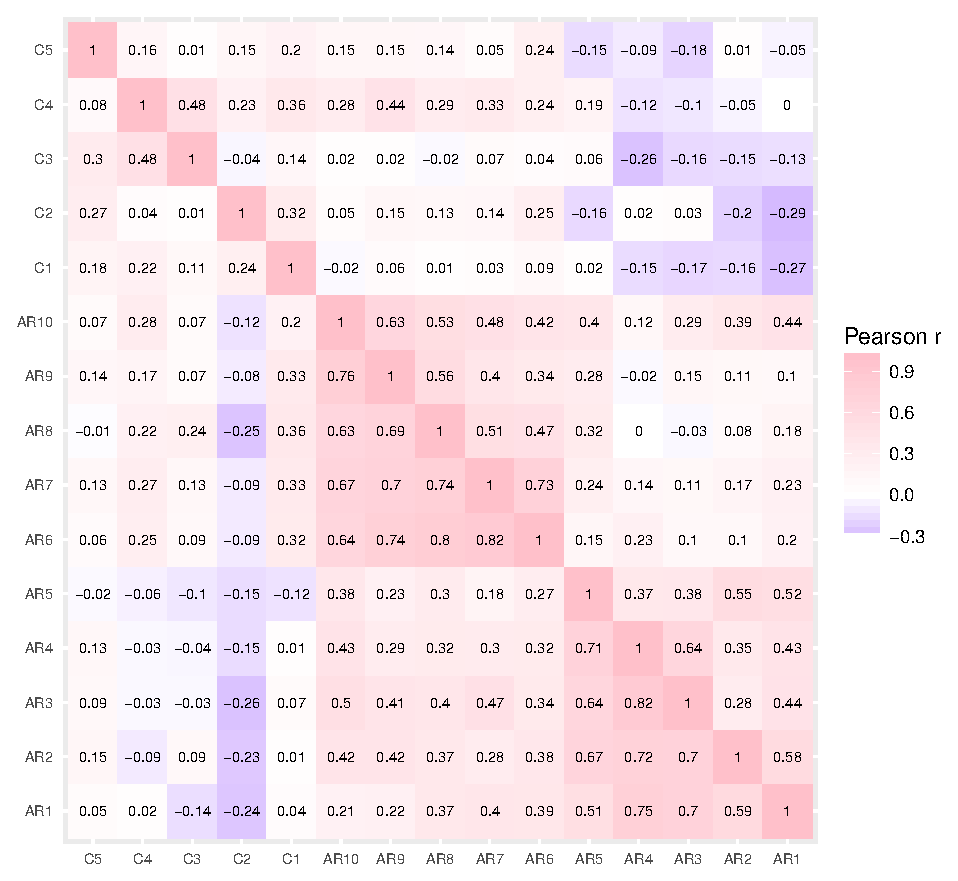
\includegraphics[width=6.7in,height=6in]{figs/em1_bayes-fig1-1}} 
\caption{Correlation matrix of data from Peters \& Levin (2008).  Correlations for the positive frame condition are below the main diagonal; correlations for the negative frame condition are above the main diagonal.  Variables include riskless attraction rating on items 1--5 (AR1--AR5); risky attraction rating on items 1--5 (AR6--AR10); and choice rating on items 1--5 (C1--C5).  Red values signify correlations closer to 1, and blue values signify negative correlations.}
\label{fig:em1:data}
\end{figure}

\subsection{Results}
Correlations between the 15 observed ratings (riskless attractiveness, risky attractiveness, choice) are presented in Figure~\ref{fig:em1:data}  (other descriptive statistics can be found in the original authors' paper). Correlations for the negative frame condition are displayed above the main diagonal, and correlations for the positive frame condition are displayed below the main diagonal.  Blue shadings imply negative correlations, and red shadings imply positive correlations.  It is seen that the riskless ratings  (AR1--AR5) generally display large correlations with one another, as do the risky ratings (AR6--AR10).  Correlations between the riskless ratings and risky ratings are also generally positive: for a given scenario, subjects generally found the risky and riskless options to be more or less appealing.  This may be because the options had the same expected value, and some subjects found the expected value to be more appealing than others. Correlations between the choice ratings (C1--C5) and the attractiveness ratings are generally smaller, and they generally differ in sign by type of option: the riskless ratings are generally negatively related to choice ratings, while the risky ratings are generally positively related. The original authors' focal hypotheses involve moderation of these  latter correlations by numeracy.

Model estimation was on the order of minutes (on our computers, two minutes or less), as opposed to seconds or hours.     We build up to the focal hypotheses by first comparing two exploratory factor models: a one-factor model and a two-factor model (i.e., a model with $m=1$ versus a model with $m=2$).  As stated previously, this comparison provides information about the nature of attraction to risky and riskless alternatives: are these attractions two extremes of a single dimension, or are they unique dimensions?  In employing the Laplace approximation to compare models, we obtain an estimated log-Bayes factor of 29.02 in favor of the two-factor model.  This implies that attraction to risky options and attraction to riskless options should be treated as separate dimensions.  Table~\ref{tab:em1:2fload} displays the posterior mean factor loadings (i.e., the estimated $\lambda$s) and reinforces this result.  The table shows that the riskless alternatives (labeled AR1 to AR5) all have large, positive loadings on the first factor and near-zero loadings on the second factor.  The risky alternatives (labeled AR6 to AR10) exhibit the converse result, with the estimated correlation between factors being  0.42. The loadings that equal exactly zero (i.e., that equal 0 instead of $0.00$) reflect identification constraints for the exploratory model; these constraints led to factor loadings that were easy to interpret, without the need for further rotation. Based on these results, we maintain a 2-factor confirmatory model for the remainder of the analyses.  This model fixes to zero the loadings that are already near zero in Table~\ref{tab:em1:2fload}: the risky alternatives on the ``Riskless'' factor, and the riskless alternatives on the ``Risky'' factor.

\begin{table}
\caption{Estimated factor loadings from the exploratory model with $m=2$. AR1 to AR5 represent attraction to the riskless options for items 1 to 5, and AR6 to AR10 represent attraction to the risky options.  Rows correspond to the two factors, labeled ``Riskless'' and ``Risky.''}
\label{tab:em1:2fload}
\centering
{\small
\begin{tabular}{lrrrrrrrrrr}\\
         &  AR1 &   AR2 &  AR3 &   AR4 &   AR5 &  AR6 &  AR7 &   AR8 &   AR9 & AR10 \\\hline
Riskless & 1.19 &  1.15 & 1.19 &  1.28 &  1.13 & 0.00 & 0.05 & -0.03 & -0.02 & 0.30 \\
Risky    & 0.00 & -0.05 & 0.00 & -0.17 & -0.06 & 1.20 & 1.14 &  1.12 &  1.11 & 0.98 \\ 
\end{tabular}}
\end{table}

We are now prepared to additionally model the impact of numeracy on attraction, along with the impacts of frame, numeracy, and attraction on choice via the model displayed in Figure~\ref{fig:em1:path}.  The results are displayed in the rightmost columns of Table~\ref{tab:em1:datcomp}, including 95\% posterior intervals and log-Bayes factors associated with different parameters.

There is a small effect of frame on riskless attraction, whereby people were more attracted to the riskless option in the positive frame condition (the condition where options were phrased in terms of ``number alive'').  The posterior interval associated with this effect hovered around zero, and the log-Bayes factor favored a model where this effect equaled zero. We also modeled effects of numeracy and numeracy-by-frame interactions on the attraction latent variables, but these effects were unsupported by both the posterior intervals and Bayes factors.

We now consider effects of frame, numeracy, and the latent attraction variables on choice.  We found the standard framing effect on choice, whereby the positive frame condition led people to prefer the riskless option.  The log-Bayes factor was around~5, with the posterior interval excluding zero. There was also a small numeracy $\times$ frame interaction: numerate subjects were less impacted by question framing as compared to less-numerate subjects.  This interaction had a posterior interval that hovered around zero, with the log-Bayes factor mildly preferring a model without the interaction.

Finally, to address the focal hypothesis, attraction ratings were positively related to choice ratings, more so for numerate subjects.   First, increases in riskless attraction were associated with preferences for the riskless option, and increases in risky attraction were associated with preferences for the risky option.  The riskless attraction latent variable had a weaker association with choice than did risky attraction, with log-Bayes factors of~1.97 and~5.15, respectively. As Figure~\ref{fig:em1:path} shows, we also included numeracy $\times$ riskless attraction and numeracy $\times$ risky attraction interactions.  The interaction term involving riskless attraction had a posterior interval that did not overlap with zero, while the interaction term involving risky attraction had a posterior interval that did overlap with zero.  The log-Bayes factor favors the model that includes the riskless interaction  (1.51) but not the risky interaction (\ensuremath{-2.79}).  This suggests a small numeracy  $\times$ riskless attraction association with choice, similar to the original authors' hypotheses.  

\begin{table}
\caption{Comparison of original (general linear model) results, 95\%   posterior intervals from the factor model,   and log(Bayes factors) from the structural equation model.  Negative log(Bayes factor) implies that the   ``no-effect'' model is preferred.  Some of the original results have been converted from $t$ statistics to $F$ statistics for uniformity.} \label{tab:em1:datcomp}
{\centering\small
\begin{tabular}{lllrr}
    Effect                    & DV            & Original                       & Posterior interval & Log(BF)          \\ \hline   
    Frame                     & AT (riskless) & $F(1, 106) =  5.2,  p < .05$   &  $(\phantom{-}0.02,\phantom{-}0.81)$   & $-0.87$ \\ % p. 440, table 2
    Frame                     & AT (risky)    & Unreported (not significant)   &  $(          -0.58,\phantom{-}0.19)$   & $-2.07$ \\ % p. 441, table 3
    NU                        & AT (riskless) & $F(1, 104) = 10.8,  p < .01$   &  $(          -0.07,\phantom{-}0.32)$   & $-3.41$ \\ % p.439, under
    NU                        & AT (risky)    & Unreported (not significant)   &  $(          -0.16,\phantom{-}0.23)$   & $-4.31$ \\ 
    NU $\times$ Frame         & AT (riskless) & $F(1, 104) =  3.9,  p = .05$   &  $(          -0.5\phantom{0},\phantom{-}0.07)$   & $-2.45$ \\ % p. 441, table 3
    NU $\times$ Frame         & AT (risky)    & Unreported (not significant)   &  $(          -0.33,\phantom{-}0.22)$   & $-4.29$ \\ 
    Frame                     & Choice        & $F(1, 104) = 18.9,  p < .001$  &  $(          -3.04,          -0.68)$   & $ 5.08$ \\ % p. 438, middle second column
    NU                        & Choice        & $F(1, 104) =  0.04, p = .85$   &  $(          -0.53,\phantom{-}0.22)$   & $-2.69$ \\ % p.438, 3.2 section. 
    NU $\times$ Frame         & Choice        & $F(1, 104) =  1.8,  p = .28$   &  $(\phantom{-}0\phantom{.00},\phantom{-}1.23)$   & $-0.8 $ \\ % p. 438, middle second column
    AT (riskless)             & Choice        & $F(1, 100) =  6.76, p < 0.01$  &  $(          -1.46,          -0.2\phantom{0})$   & $ 1.97$ \\ % p. 442, t statistic
    AT (risky)                & Choice        & $F(1, 100) =  7.29, p < 0.01$  &  $(\phantom{-}0.36,\phantom{-}1.85)$   & $ 5.15$ \\ % p. 442,t statistic
    NU $\times$ AT (riskless) & Choice        & $F(1, 100) =  9.6,  p = .002$  &  $(          -0.92,          -0.12)$   & $ 1.51$ \\ % p. 441, second column
    NU $\times$ AT (risky)    & Choice        & $F(1, 100) =  4.4,  p = .04$   &  $(          -0.09,\phantom{-}0.59)$   & $-2.79$ \\ \hline % p. 441, second column
\end{tabular}}\\[6pt]
\noindent Note: DV = Dependent variable. NU = Numeracy. AT = Attraction.
\end{table}

\subsection{Discussion}
 We now discuss some general issues associated with the results in  Table~\ref{tab:em1:datcomp}, along with some limitations of the current analyses.  

\paragraph{Prior Sensitivity and Comparison} Focusing on results in Table~\ref{tab:em1:datcomp}, the magnitude of the Bayes factors is impacted by the prior distributions used (for the model here, prior distributions with smaller variances generally produce larger Bayes factors).   This property of Bayes factors is known, and it has been the subject of both praise and criticism \cite{liuait08,van10}.  The fact that Bayes factors are sensitive to choice of prior distribution is helpful in that they summarize the data while also accounting for our previous knowledge of the phenomenon under study.  Others point out that, if one needs to surpass a Bayes factor threshold for a journal publication (similar to $p<.05$), then it is disconcerting that the threshold can be met by manipulating the prior distribution.  To address this issue, one can fit the model under multiple prior distributions to examine the results' sensitivities.

We can further use Table~\ref{tab:em1:datcomp} to compare results arising from the Bayesian models to those of the original authors.  The third column of the table displays the original authors' ANOVA-based results.  Some of these results are not based on exactly the same data as our results, because the original authors sometimes focused on three of the five scenarios and sometimes aggregated data (whereas we consistently include all five scenarios).  Nevertheless, we see that the posterior intervals and Bayes factors often agree with the ANOVA results, in that intervals fail to overlap with zero and log-Bayes factors are positive when $p$-values are small.  When there are disagreements, the Bayes factors and posterior intervals appear to be more conservative than the other measures.

There are also a few situations where the posterior intervals fail to overlap with zero, yet the Bayes factors favor a model that excludes the effect. These different conclusions stemming from posterior intervals versus Bayes factors arise from their different intents: posterior intervals summarize the value of a single model parameter, while Bayes factors signify whether or not the associated parameter(s) generally improve our model. While the former are readily interpreted and may be more familiar to researchers (due to the similarity between posterior intervals and confidence intervals), the latter seems more useful for summarizing the extent to which a parameter is generally important to one's theory (somewhat similarly to a frequentist likelihood ratio test). Bayes factors additionally account for the complexity afforded to us by extra model parameters, which is relevant here because some types of SEM parameters may afford us more complexity than other types. For further discussion of Bayes factors and of model complexity, see \citeA{jefber92} and \citeA{spismi82}.

\paragraph{Limitations} If the focus of this paper were risky choice (as opposed to Bayesian latent variable models), further model extension and study would be warranted.  The model used here posits three separate latent variables for risky attraction, riskless attraction, and choice.  Conditional on these latent variables, the observed variables are posited to be independent.  This assumption is likely to be incorrect  for observed variables stemming from the same problem.  That is, even after conditioning on the latent variables, there may remain a correlation between the three observed variables associated with any one  problem (e.g., the variables labeled AR1, AR6, and C1 in Figure~\ref{fig:em1:path}).  To account for these issues, we can allow the residual terms associated with these three variables (E1, E6, and E11) to be correlated.  The introduction of residual correlations poses a difficult problem for Bayesian SEM estimation \cite{barmcc00,chigre98,paldun07}, though model estimation  is possible \cite<e.g.,>{mutasp12} and will become easier in the future \cite<e.g.,>{merros16}.

Aside from residual correlations, several issues deserve more attention than they received here.  First, it would be useful to include more descriptive statistics that supplement the model. \citeA{petlev08} provided many tables that are useful along these lines.  Second, it would be useful to study the absolute fits of the models in addition to the relative fits.  This may involve posterior predictive checks \cite<e.g.,>{gelcarste04} or calculation of a Bayes factor comparing the proposed models to saturated models (i.e., multivariate normal models with a free  parameter for each mean and covariance).  Finally, the statistical issue of suppression may be considered in more detail.  The SEM from Figure~\ref{fig:em1:path} involves two positively-related latent variables predicting a third latent variable with opposite signs.  This can lead to instability in the associated regression weights and standard errors.  While the signs of the regression weights involving latent variables are the same as the majority of relevant, observed-variable correlations in Figure~\ref{fig:em1:data}, some instability may still exist.

In the General Discussion below, we provide detail about further model extensions, uses, and needs. 

\section{General Discussion}
In this paper, we have demonstrated the utility of applying Bayesian latent variable models to multivariate experimental psychology data.  We first provided background on factor analysis models, structural equation models, and issues specifically related to Bayesian estimation of these models.   We then considered some model extensions and applied them to data from a decision making experiment on risky choice.  The models allowed us to draw conclusions across multiple stimuli in a unified manner, removing the need for data aggregation and for separate, stimulus-specific analyses.  Bayesian methods further allowed us to easily estimate models with latent variable interactions, which are difficult to estimate via ML methods.  In the paragraphs below, we address additional Bayesian model extensions and needs.  These include general comparisons to ML models, considerations of exploratory factor analysis, and cognitive psychometric models.

\paragraph{Bayesian versus ML} Advantages of the Bayesian approach to structural equation modeling include easy extension to complex situations, along with non-asymptotic estimates of the variability in parameter estimates.   Expanding on the former point, the methods described here were easily extended to handle latent variable interactions, and they are also easily extended to handle models with both continuous and ordinal observed variables.  In particular, \citeA{sonlee12b} provide a tutorial on Bayesian  estimation of these types of models, with further details in their book \cite{sonlee12}.  These methods are very powerful because they provide a single framework for estimating many structural equation models that a researcher may conceptualize.  This framework is not necessarily the best for building an intuition of structural equation models, however, because it is so general.  Researchers' desired models can often be written in a manner that is more concise than the general framework.

Disadvantages of Bayesian structural equation models, as compared to ML models, lie in model specification and estimation.  Model specification in, e.g., JAGS is very different from model specification in traditional ML software like Mplus or LISREL, so that users coming from these traditions will find that their prior software experience is not terribly helpful. Relatedly, Bayesian methodology has more ``moving parts,'' including prior distribution specification and assessments of model convergence.  These represent new topics for users of ML software, but we are optimistic that users can master the new topics.  

\paragraph{Bayesian exploratory factor analysis} Bayesian methods offer novel ways to estimate exploratory factor models.  In this paper, we always fixed specific parameters to zero in order to identify model parameters.  If the factor model is exploratory, we could then rotate model parameters' (the $\lambda$s) posterior means to  have a more-interpretable structure.  This is a two-step process, just like the ML case: we first estimate the model, and we then rotate parameters.  Under the Bayesian approach, we could simultaneously rotate and sample the factor loading matrices at each iteration of the MCMC algorithm, which may lead to more-interpretable solutions than the ML algorithm (which can only use the single set of factor loadings arising from the ML estimates).  

Related methods have been the focus of recent work.  In particular, \citeA{pee12b} describes a method by which factor models with multiple  values of $m$ are simultaneously estimated, rotated, and compared to one another via marginal likelihoods (the building blocks of Bayes factors).  \citeA{confru14} propose a method whereby the value of  $m$ is allowed to change from iteration to iteration, with the possibility that some latent traits are associated with no observed variables.  Importantly, the latter  authors assume that every observed variable has a nonzero loading associated with only one latent trait; this assumption is restrictive and results in a model that, using the definitions in this paper, would be called ``confirmatory'' instead of ``exploratory.''  Finally, \citeA{rocgeo14} propose an alternative method whereby $m$ is set to a large value, and ``spike-and-slab'' priors are used to enforce simplicity of the $\bm{\Lambda}$ matrix.  These prior distributions fix weak loadings to zero, so that smaller values of $m$ are obtained by fixing to zero all loadings associated with a latent trait.  This method is computationally difficult but appears promising for future application.

\paragraph{Cognitive psychometric models} The methods described here are highly related to the development of {\em cognitive} latent variable models \cite<e.g.,>{nunsri15,turfor13,turvan15,van14},  where the latent variables are used to tie multiple types of data (response time, BOLD response, survey data, etc) together in a single model.  For example, in Vandekerckhove's application, a diffusion model was used to describe response times from an executive functioning task.  Participants also completed two depression scales, with the latent variables in the model predicting both the depression scales and diffusion model parameters.  This allowed for novel information about specific aspects of performance on the response time task that are related to the depression scales.  Cognitive psychometric models generally offer new avenues for  combining psychometric knowledge with cognitive modeling \cite<also see, e.g.,>{tuedeb05,vanmol11}. 

The model extensions mentioned here, coupled with  computational advances in model estimation and increased communication between experimental psychologists and psychometricians,  yield fruitful prospects for the use of Bayesian latent variable models in cognitive science.  We encourage readers to explore these prospective models and the novel inferences that they can provide.

\section*{Computational Details}

All results were obtained using the \proglang{R}~system for statistical computing \cite{Rprog}  version~3.2.3 and \proglang{JAGS}~software for Bayesian computation version 3.4.0, employing the helper package \pkg{rjags}~4-5 \cite{plu14}. \proglang{R}~and the package \pkg{rjags} are freely available under the General Public License~2 from the Comprehensive \proglang{R} Archive Network at \url{http://CRAN.R-project.org/}. \proglang{JAGS} is freely available under the General Public License~2 from Sourceforge at \url{http://mcmc-jags.sourceforge.net/}.   \proglang{R}~and \proglang{JAGS}~code for replication of our results is available at \url{http://semtools.R-Forge.R-project.org/}.

\bibliographystyle{apacite}
\bibliography{em1}
